% Chapter Template

\chapter{Graph-Based Structural Output Learning} % Main chapter title
\label{Chapter3} % Change X to a consecutive number; for referencing this chapter elsewhere, use \ref{ChapterX}
\lhead{Chapter 3. \emph{Graph-Based Structural Output Learning}} % Change X to a consecutive number; this is for the header on each page - perhaps a shortened title



\rule{\textwidth}{0.4pt} \\[0.5cm]
\textit{``To learn without thinking is blindness; to think without learning is idleness. "}

\begin{flushright}
Confucius
\end{flushright}
\rule{\textwidth}{0.4pt} 


%----------------------------------------------------------------------------------------
%	SECTION 1
%----------------------------------------------------------------------------------------

\section{Conditional Random Field}
\label{sec:crf}
For instance, in a multi-label learning case, input $\mathbf{x}\in{\mathbb{R}^D}$ is a $D$-dimensional real-value vector, output $\mathbf{y}\in\mathbb{B}^L$ is a $L$-dimensional 
binary vector with a component $y_{l:l\in[1:L]}$ denoting the presence of the $l$th label. A \emph{Markov random field} (MRF) $p(\mathbf{x,y})$ can be defined by a  domain expert, or learned from 
existing training data, with a graph structure and 
associated potential functions, which are supposed to reconstruct the generative process of $\{\mathbf{x,y}\}: p(\mathbf{x,y})=p(\mathbf{x})p(\mathbf{y}|\mathbf{x})$. 
As for the prediction task, the conditional probability 
$p(\mathbf{y|x})=\frac{p(\mathbf{x,y})}{\sum_\mathbf{y} p(\mathbf{x,y})}$ can be derived, or more straightforwardly, 
$\mathbf{y}^*=\arg\max_{\mathbf{y}}p(\mathbf{y|x})=\arg\max_{\mathbf{y}}p(\mathbf{x,y})$ (\emph{e.g.} by using max-product algorithm). However, it was realised that for the task $\mathbf{x}\to\mathbf{y}$, the only desired
component is $p(\mathbf{y|x})$; it is wast to expend effort in modeling $p(\mathbf{x})$, which is not relevant anyway. Consequently, \emph{conditional random field} (CRF) was proposed \citep{CRF} as 
a discriminative model by learning only the conditional probability $p(\mathbf{y|x})$. One strength of CRFs is that it can include arbitrarily complex features (\emph{e.g.} higher order dependencies) 
of $\mathbf{x}$, which is intractable in MRFs. According to empirical study in \citep{Kumar03,CRF}, CRFs outperform MRFs in many practical applications. 

At first, the definition of conditional random fields (CRFs) give as \citep{CRF}: 
\begin{definition}
    Let $G=(V,E)$ be a graph ($V$ are vertices and $E$ are edges) such that $\mathbf{y}=\{y_v\}_{v\in V}$, so that $y$ is indexed by the vertices of $G$. Then $(\mathbf{x,y})$ is a 
        conditional random field in case, when conditioned on $\mathbf{x}$, the random variables $\{y_v\}_{v\in V}$ obey the Markov property with respect to 
    the graph $G$.   
\label{def:CRF}
\end{definition}
Assume that the joint conditional probability $p(\mathbf{y|x})$ is defined in an exponential form: 
\begin{equation}
    p(\mathbf{y|x})=\frac{\exp(\mathbf{w}^\top \boldsymbol{\phi}(\mathbf{x,y}))}{\mathbf{Z(w)}}
\end{equation}
where $\mathbf{x}\in\mathcal{X},\mathbf{y}\in\mathcal{Y}$, $\boldsymbol{\phi}(\mathbf{x,y})\in\mathbb{R}^K$ is a collection of $K$ predefined, task-specific potential functions  (or feature vectors)
$\boldsymbol{\phi}(\mathbf{x,y})=[\phi_1(\mathbf{x,y}),\cdots \phi_K(\mathbf{x,y})]^\top$, $\mathbf{w}\in\mathbb{R}^K$ is the parameter vector,  
$\mathbf{Z(w)}$ is the partition function for normalization $\mathbf{Z(w)}=\sum_{\mathbf{y}\in\mathcal{Y}} \exp(\mathbf{w}^\top \boldsymbol{\phi}(\mathbf{x,y}))$. 

As a probabilistic model, one CRF is usually 
learned via \emph{maximum likelihood estimation} (MLE) or \emph{maximum a posterior} (MAP) \citep{Kumar03,CRF,Accelerated_CRF}. 
Meanwhile, inspired by the margin notion which has been exploited in successful binary classifiers, \emph{e.g.} Support Vector Machine (SVM),  
an alternative discriminative training scheme of CRFs is maximizing the margin between 
the $p(\mathbf{y|x})$ of the desired $\mathbf{y^*}$ and the best runner-up $\mathbf{y}^{**}$  in their $\log$ domains. The CRFs trained with this 
margin
are referred to as 
\emph{Max-Margin Markov Networks} (M$^3$Ns) \citep{Taskar03}. 
On the one hand, similarly to regular SVM, \emph{kernel tricks} can be used in the dual form of M$^3$N, in which way, the original inputs and/or outputs are implicitly mapped into a higher 
dimensional \emph{reproducing kernel Hilbert space} (RKHS) (\emph{e.g.} polynomial kernels used in \citep{Taskar03}).     
On the other hand, different from regular SVM, the \emph{quadratic programming} 
(QP) problem associated with M$^3$Ns (in both primal and dual form) has exponential number of constraints. 
Although it can be simplified by exploiting interesting properties within forest-structured outputs \citep{Taskar03},  
for highly connected graphs, the learning is intractable.      
Obviously, although CRF and  M$^3$Ns offer almost equivalent modeling capabilities for a given machine learning task, two rather different loss functions are 
employed in them. However, it can be revealed that MAP and max-margin learning schemes are, to large extent, related. 
%-----------------------------------
%	SUBSECTION 1
%-----------------------------------
\subsection{Maximum Likelihood Estimation}
\label{subsec:MLE}
Given a training dataset $\mathcal{D}=\{\mathbf{x}^{(i)},\mathbf{y}^{(i)}\}_{i=1}^M$, a CRF can be learned via maximum likelihood estimation (MLE):
\begin{equation}
    \begin{array}{rl}
        \mathbf{w}^* =& \arg\max_{\mathbf{w}} \frac{1}{M}\sum_{i=1}^M \log p(\mathbf{y}^{(i)}|\mathbf{x}^{(i)}) \\
                     =& \arg\max_{\mathbf{w}} \frac{1}{M}\sum_{i=1}^M \{\mathbf{w}^\top \boldsymbol{\phi}(\mathbf{x}^{(i)},\mathbf{y}^{(i)}) -\log \sum_{\mathbf{y}\in\mathcal{Y}} \exp(\mathbf{w}^\top \boldsymbol{\phi}(\mathbf{x}^{(i)},\mathbf{y}))\}
    \end{array}
    \label{equ:MLE}
\end{equation}
Meanwhile, usually, in order to enhance the generalization properties, a prior on $p(\mathbf{w})\propto \exp(-\frac{\mathbf{w}^2}{\sigma^2})$ is added in (\ref{equ:MLE}) to penalize the complexity of $\mathbf{w}$, which 
results in the maximum a posterior (MAP) solution:
\begin{equation}
    \begin{array}{rl}
        \mathbf{w}^* =& \arg\max_{\mathbf{w}}  -\frac{\mathbf{w}^2}{\sigma^2} +\frac{1}{M}\sum_{i=1}^M \{\mathbf{w}^\top \boldsymbol{\phi}(\mathbf{x}^{(i)},\mathbf{y}^{(i)}) -\log \sum_{\mathbf{y}\in\mathcal{Y}} \exp(\mathbf{w}^\top \boldsymbol{\phi}(\mathbf{x}^{(i)},\mathbf{y}))\}  \\ 
                     =& \arg\min_{\mathbf{w}} \frac{1}{2} ||\mathbf{w}||^2+  \frac{C}{M}\sum_{i=1}^M \mathcal{L}^{MAP}_i 
    \end{array}
    \label{equ:MAP}
\end{equation}
where $\mathcal{L}_i^{MAP}$ is the negative log-likelihood of the $i$th training instance:  
\begin{equation}
    \mathcal{L}^{MAP}_i=\log \sum_{\mathbf{y}\in\mathcal{Y}} \exp(\mathbf{w}^\top \boldsymbol{\phi}(\mathbf{x}^{(i)},\mathbf{y}))-\mathbf{w}^\top \boldsymbol{\phi}(\mathbf{x}^{(i)},\mathbf{y}^{(i)})
    \label{equ:MAP_loss}
\end{equation}
and $C=\frac{\sigma^2}{2}$ is a trade-off parameter to balance the regularization term $\frac{1}{2} ||\mathbf{w}||^2$ and average loss $\frac{1}{M}\sum_{i=1}^M \mathcal{L}^{MAP}_i$. A good property 
of (\ref{equ:MAP}) is that it is convex with respect to $\mathbf{w}$. 
\begin{proposition}
    The objective function of maximum a posterior in learning CRFs is convex.
\label{pro:MAP_convex}
\end{proposition}

\begin{proof}
    The second order derivative of $\log \sum_{\mathbf{y}} \exp(\mathbf{w}^\top \boldsymbol{\phi}(\mathbf{x}^{(i)},\mathbf{y}))$ with respect to 
    $\mathbf{w}$ is:
    \begin{equation}
    \frac{d^2 \log \sum_{\mathbf{y}} \exp(\mathbf{w}^\top \boldsymbol{\phi}(\mathbf{x}^{(i)},\mathbf{y}))}{d \mathbf{w}^2}=\mathbf{Cov}_{p(\mathbf{y}|\mathbf{x}^{(i)};\mathbf{w})}\boldsymbol{\phi}(\mathbf{x}^{(i)},\mathbf{y})
    \end{equation}
    where $\mathbf{Cov}_{p(\boldsymbol{\rho})}f(\boldsymbol{\rho})$ denotes the covariance of $f(\boldsymbol{\rho})$ under the probability $p(\boldsymbol{\rho})$. 
    Since the covariance function is always positive semidefinite, $\log \sum_{\mathbf{y}} \exp(\mathbf{w}^\top \boldsymbol{\phi}(\mathbf{x}^{(i)},\mathbf{y}))$ is convex. In addition, 
    $-\mathbf{w}^\top \boldsymbol{\phi}(\mathbf{x}^{(i)},\mathbf{y}^{(i)})$ is linear (thus also convex), and $\frac{1}{2} ||\mathbf{w}||^2$ is convex. Therefore, 
    (\ref{equ:MAP}) (the sum of convex components) is convex.  
\end{proof}
Because of the convexity of the objective function, any local minimum is also global minimum, and gradient descent can be employed to find the unique solution 
$\mathbf{w}^*$ with the negative gradient computed as: 
\begin{equation}
    \Delta \mathbf{w}_t=\frac{C}{M}\sum_{i=1}^M(\boldsymbol{\phi}(\mathbf{x}^{(i)},\mathbf{y}^{(i)})-\mathbb{E}_{p(\mathbf{y}|\mathbf{x}^{(i)};\mathbf{w}_t)} \boldsymbol{\phi}(\mathbf{x}^{(i)},\mathbf{y}))-\mathbf{w}_t 
\label{equ:gradient_MAP}
\end{equation}
where $\mathbb{E}_{p(\boldsymbol{\rho})}f(\boldsymbol{\rho})$ is the expectation of $f(\boldsymbol{\rho})$ under the probability $p(\boldsymbol{\rho})$.
The difficulty of computing (\ref{equ:gradient_MAP}) is the expectation term because its complexity grows exponentially. For example, in multi-label 
learning case introduced in section \ref{sec:crf}, $|\mathcal{Y}|=2^L$. 
Therefore, when $|\mathcal{Y}|$ is relatively large in practice, some approximations are used, \emph{e.g.} by using \emph{mean field} (MF), \emph{loopy 
belief propagation} (LBP) or \emph{pseudo likelihood} (PL) \citep{LBP, Kumar03,CRF,Accelerated_CRF}.  



\subsection{Max-Margin Markov Network}
\label{subsec:MMMN}
The max-margin principle used in binary classifier, \emph{e.g.} Support Vector Machine (SVM), has been proven theoretically and empirically \citep{Vapnik} superior to others.        
The margin notion was generalized to learn structured outputs in \citep{Taskar03} and \citep{StructSVM}. More concretely, they proposed to learn CRFs by maximizing the margin 
between the $p(\mathbf{y|x})$ of the desired $\mathbf{y^*}$ and the best runner-up $\mathbf{y}^{**}$ in log domain. The CRFs trained with maximum margin are referred to as 
max-margin Markov networks (M$^3$N) \citep{Taskar03}.  The objective function of M$^3$N can be written out as: 
\begin{equation}
    \begin{array}{rl}
        & \arg\min_{\mathbf{w},\xi_{i:i\in[1,M]}}  \frac{1}{2} ||\mathbf{w}||^2 +\frac{C}{M} \sum_{i=1}^M \xi_i \\
   s.t. &\forall i, \forall y\in\mathcal{Y}/\mathbf{y}^{(i)}: \xi_i\geq0, \mathbf{w}^\top (\boldsymbol{\phi}(\mathbf{x}^{(i)},\mathbf{y}^{(i)})-\boldsymbol{\phi} 
        (\mathbf{x}^{(i)},\mathbf{y}))\geq 1-\frac{\xi_i}{d(\mathbf{y}^{(i)},\mathbf{y})}
    \end{array}
    \label{equ:MMMN}
\end{equation}
where $\xi_i$ are slack variables for the relaxation of 
max-margin, and $d(\mathbf{y}^{(i)},\mathbf{y})\geq0$ is a measure of dissimilarity between $\mathbf{y}^{(i)}$ and $\mathbf{y}$ 
(\emph{e.g.} hamming distance used in the multilable learning case). The term $\frac{\xi_i}{d(\mathbf{y}^{(i)},\mathbf{y})}$ is to rescale 
slack variables by the dissimilarities between corresponding $\mathbf{y}^{(i)}$ and others. 
Obviously, (\ref{equ:MMMN}) is a quadratic programming (QP)  problem with exponential number of 
constraints. Similarly to SVM, (\ref{equ:MMMN}) can be converted to its dual form, of which some interesting properties can be exploited 
to simplify the computation 
for forest-structured outputs (\emph{i.e.} singly-connected graphs). However, for highly-connected graphs, exact learning is intractable.  
An advantage of the dual form of M$^3$N is that it enables the use of \emph{kernel methods}, which can implicitly project 
$\boldsymbol{\phi}(\mathbf{x},\mathbf{y})$ to 
a higher dimensional Hilbert feature space. Defining $\boldsymbol{\phi}(\mathbf{x},\mathbf{y})$  with kernel methods was more exploited in Structural SVM \citep{StructSVM} (see section \ref{sec:SSVM}). 
Usually quadratic or cubic kernels are used and yield promising results \citep{Taskar03}. 
Correspondingly, 
explicitly feature map of $\boldsymbol{\phi}(\mathbf{x},\mathbf{y})$  can be constructed via two-degree and three-degree polynomials in the primal form of M$^3$Ns.  

The second constraint in (\ref{equ:MMMN}) can be written in a more compact form: 
$\max_{\mathbf{y}\in\mathcal{Y}} \{d(\mathbf{y}^{(i)},\mathbf{y})-{\mathbf{w}^\top} (\boldsymbol{\phi}(\mathbf{x}^{(i)},\mathbf{y}^{(i)})-\boldsymbol{\phi} 
        (\mathbf{x}^{(i)},\mathbf{y})) d(\mathbf{y}^{(i)},\mathbf{y}\}\leq \xi_i$. 
In addition, we can rescale $\mathbf{w}$ ($\mathbf{w}\gets \mathbf{w}d(\mathbf{y}^{(i)},\mathbf{y})$)
%; it will not affect the solution of Eq. (\ref{equ:MMMN}) 
%because the magnitude of $\mathbf{w}$ will be minimized anyway \citep{Taskar03,OnlineMKL}
. Then, instead of rescaling slack variables, we rescale margin to be the same level as 
$d(\mathbf{y}^{(i)},\mathbf{y})$.  
Therefore, Eq. (\ref{equ:MMMN}) can be reformulated in a similar form as Eq. (\ref{equ:MAP}):
\begin{equation}
        \mathbf{w}^* = \arg\min_{\mathbf{w}} \frac{1}{2} ||\mathbf{w}||^2+ \frac{C}{M}\sum_{i=1}^M \mathcal{L}^{Margin}_i 
    \label{equ:MMMN_compact}
\end{equation}
where 
\begin{equation} 
    \mathcal{L}^{Margin}_i=\max_{\mathbf{y}\in\mathcal{Y}} \{d(\mathbf{y}^{(i)},\mathbf{y})+ \mathbf{w}^\top\boldsymbol{\phi} 
        (\mathbf{x}^{(i)},\mathbf{y})\} -\mathbf{w}^\top\boldsymbol{\phi}(\mathbf{x}^{(i)},\mathbf{y}^{(i)})
\label{equ:MMMN_loss}
\end{equation}





%----------------------------------------------------------------------------------------
%	SECTION 2
%----------------------------------------------------------------------------------------
\section{Training Undirected Graphical Models with Persistent Sequential Monte Carlo}

\begin{shaded}
{\Huge II.} \textbf{Hanchen Xiong}, Sandor Szedmak, Justus Piater. {\it Towards Maximum Likelihood: Learning Undirected Graphical Models using Persistent Sequential Monte Carlo}, The 6th Asian Conference on Machine Learning (ACML2014), 
\end{shaded}
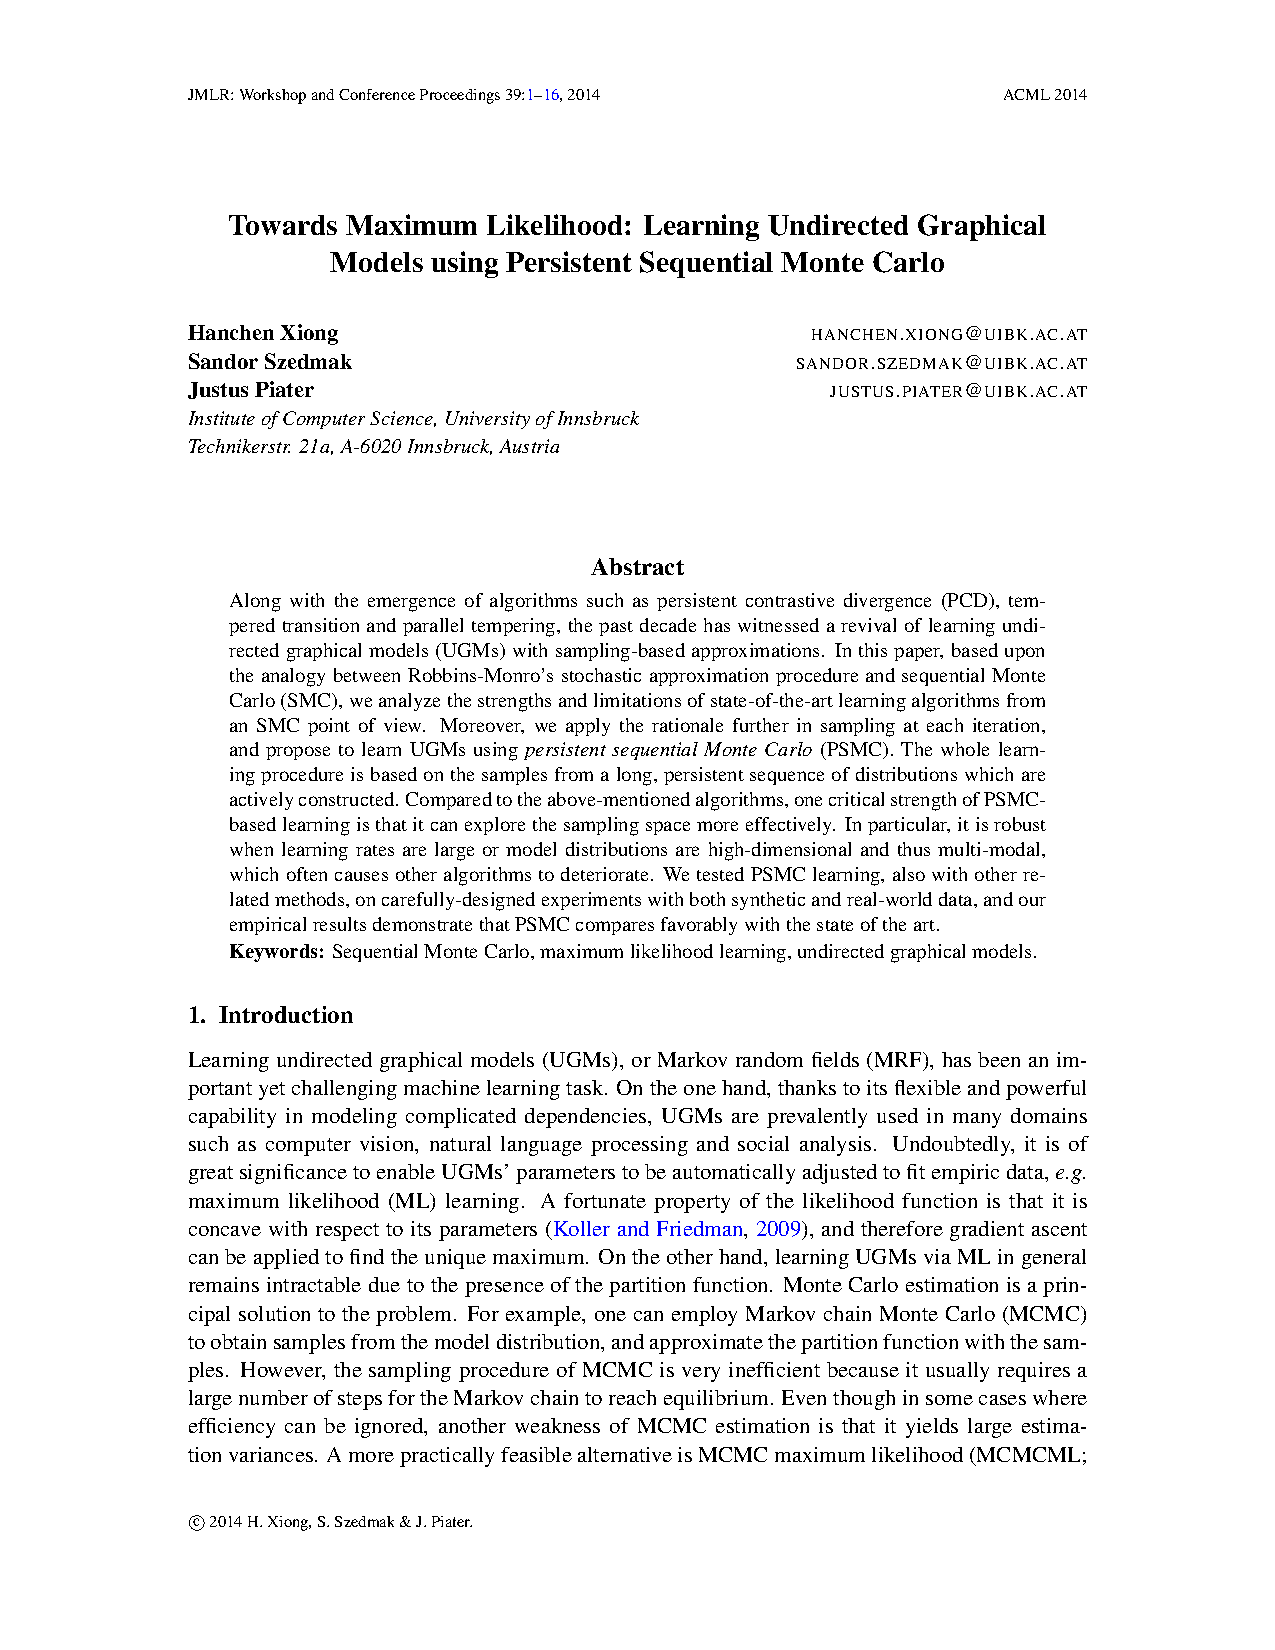
\includepdf[offset=3cm -2.5cm, scale=1, pages=-,pagecommand={\pagestyle{fancy}}]{./Papers/Xiong-2014-ACML.pdf}

\subsection {Training Conditional Random Fields for Image Annotation and Image Segmentation}
In this section we present some evaluations and comparison of different learning algorithms on two practical tasks: \emph{multi-label learning} and \emph{image 
segmentation}. Different from previous experiments where generative models were learned, here we trained discriminative models. Therefore, two 
conditional random fields were employed. Generally speaking, let us denote $\mathbf{x}$ as input and $\mathbf{y}\in \mathcal{Y}$ as output, and our target is to 
learn an UGM:  
\begin{equation}
	p(\mathbf{y}|\mathbf{x})=\frac{\exp(\boldsymbol{\theta}^\top \phi(\mathbf{y},\mathbf{x}))}{\mathbf{Z}}
\end{equation}
where the partition function $\mathbf{Z}$ is
\begin{equation}
	\mathbf{Z}=\sum_{\mathbf{y}\in\mathcal{Y}}\exp(\boldsymbol{\theta}^\top \phi(\mathbf{y},\mathbf{x}))
\end{equation}
where $\phi(\mathbf{y},\mathbf{x})$ is defined based on task-oriented dependency structure. Note that the partition function $\mathbf{Z}$ is computed by 
marginalizing out only $\mathbf{y}$ because our interest is a conditional distribution. Six algorithms 
were implemented: PCD-$H$, PCD-1, PT, TT, SMC and PSMC. Similar setups were used for all algorithms as the previous section.  
Learning rate $\eta_t=\frac{1}{10+0.1*t}$ was used and 100 iterations were run. For each input $\mathbf{x}$, 
the size of particle set $\{ \hat{\mathbf{y}}^{(s)}\}$ is 200.  Similar to other supervised learning schemes, a regularization $\frac{1}{2}||\boldsymbol{\theta}||^2$ 
was added and a trade-off parameters was tunned via $k$ folder cross-validation ($k=4$).  

It is worth mentioning that better results can be expected in both experiments by running more iterations, using better learning rates or exploiting 
feature engineering. However, our purpose here is to compare different learning algorithms under the some conditional instead of defeat state-of-the-art 
results in multi-label learning study and image segmentation study respectively. Therefore, we saved our effort in tunning algorithms and constructing 
sophisticated features. 

\subsubsection{Multi-Label Learning}
In multi-label learning, inter-label dependency is rather critical. Assume that input $\mathbf{x}\in \mathbb{R}^d$ and there are $L$ labels (\emph{i.e.} $\mathbf{y}\in\{-1,+1\}^L$), here we modeled all pairwise dependencies among $L$ labels, and therefore 
the constructed conditional random field is:
\begin{equation}
	p(\mathbf{y}|\mathbf{x})=\frac{\exp(\mathbf{y}^\top\mathbf{W}_E \mathbf{y}+\mathbf{y}^\top \mathbf{W}_v \mathbf{x})}{\mathbf{Z}}
	\label{equ:scene_model}
\end{equation}
where $\mathbf{W}_E\in \mathbb{R}^{L\times L}$ captures pairwise dependencies among $L$ labels while $\mathbf{W}_v\in \mathbb{R}^{L\times d}$ reflects the 
dependencies between input $\mathbf{x}$ and all individual labels.   
In the test phase, with learned $\mathbf{W}_E$ and $\mathbf{W}_v$, for a test input $\mathbf{x}^\dagger$, we predict the corresponding $\mathbf{y}^\dagger$ with 
100 rounds of gibbs sampling based on (\ref{equ:scene_model}).  

In our experiment, we used popular \emph{scene} database \citep{scene_database}, where scene images are associated with a few semantic labels. In the database, 
there are 1121 training instances and 1196 test instances.  In total there are 6 labels ($L=6$) and a 294 dimensional feature were extracted from each image         
($\mathbf{x}\in\mathbb{R}^{294}$). Readers are referred to \cite{scene_database} for more details about the database and feature extraction.  

We evaluated the performance of multi-label learning using \emph{precision} (P), \emph{recall} (R), and the \emph{F1} measure (F). For each label, the precision is 
computed as the ratio of the number of images assigned the label correctly over the total number of images predicted to have the label, while the recall is the number of images 
assigned the label correctly divided by the number of images that truly have the label. Then precision and recall are averaged across all labels. Finally, the F1 measure is calculated as 
$F=2\frac{P\times R}{P+R}$.
The results of all six algorithms are presented in Table \ref{tab:scene_results}.     
The average number temperatures in PSMC is around 5, so PCD-5 was implemented. Also 5 temperatures were use in PT and TT.    
We can see that PSMC yields the best F1 measure 75.1, followed by PT and SMC with 74.6 and 73.4 respectively. The results of PCD-5 and TT             
are relative worse, while PCD-1 is the worst.  


\begin{table}
	\label{tab:scene_results}
	\center
\begin{tabular}{cccc} 
\Xhline{2\arrayrulewidth} \\ 
       & Precision($\%$) & Recall($\%$) & F1($\%$) \\ \hline 
 PCD-1 & 57.7            & 59.3         & 58.5 \\
 PCD-5 & 70.3            & 72.6         & 71.4 \\
 TT    & 70.0            & 67.5         & 68.7 \\
 PT    & {\bf 72.2}      & 77.1         & 74.6 \\
SMC    & 71.7            & 75.1         & 73.4 \\
PSMC   & 71.9            & {\bf 78.5}   & {\bf 75.1} \\ 
\Xhline{2\arrayrulewidth}
 \end{tabular}
 \caption{A comparison of six learning algorithms on multi-label learning. }
\end{table}

\subsubsection{Image Segmentation} 
Image segmentation essentially is a task to predict the semantic label of all image pixels or blocks.    
Inter-label dependences within neighbourhood are usually exploited in image segmentation. For instance, by dividing an image into equal size and non-overlapping 
blocks, the label of a block does not only depend on the appearance of the block, but also the labels of its neighbouring blocks. For simplicity, here 
we only consider binary labels. In addition, we assume that blocks and inter-label dependencies are position irrelevant. Therefore, a conditional random filed can 
be constructed as:               
\begin{equation}
	p(\mathbf{y}|\mathbf{x})=\frac{\exp(\sum_{u,v\in E}y_u W_e y_v+\sum_{v\in V} y_v \mathbf{w}_v^\top \mathbf{x}_v) }{\mathbf{Z}}
\end{equation}
where $y_v\in\{-1,+1\}$, $E$ denotes the set of all edges connecting neighbouring blocks, $W_e\in\mathbb{R}$ encodes the dependency between neighbouring labels, $V$ denotes the set of all 
block's labels and $\mathbf{w}_v\in \mathbb{R}^{d\times 1}$ encodes the dependency between block label and its appearance which is represented by a $d$-dimensional feature $\mathbf{x}_v\in\mathbb{R}^d$.    
Similar to the multi-label experiment, desired labels are predicted via 100 round gibbs sampling in test phase.      

In our experiment, we used the binary segmentation database from \cite{img_seg_database}, where each image is divided into non-overlapping blocks of 
size $16\times16$ and each block is annotated with either ``man-made structure" (MS) or ``nature structure" (NS). 
Overall, there are 108 training images and 129 test images. The training set contains 3004 MS blocks and 36269 NS blocks, while the test set 
contains 6372 MS blocks and 43164 NS blocks.
For each block, its appearance is 
represented by a 3-dimensional features which includes the mean of gradient magnitude, the 'spikeness' of the count-weighted histogram of gradient orientations, 
the angle between the most frequent orientation and the second most frequent orientation. The feature was designed to fit this specific application.        
More explanation of the database and feature design can be found in \cite{img_seg_database}. 


We found that the average number of temperatures in PSMC is 20, therefore PCD-20 was run and 20 temperatures were used in TT and PT. We quantify the segmentation performance of 
six algorithms with confusion matrices, which are presented in Figure \ref{fig:img_seg_results}. We can see that PSMC outperforms all others (by checking the diagonal entries of confusion matrices).      
For qualitative comparison, an example image and corresponding segmentations are shown in Figure \ref{fig:img_seg_example}.  It can be seen that the segmentation by PSMC is closer to the ground truth 
compared to others. 
\begin{figure}[t!] 
    \centering
    \subfigure{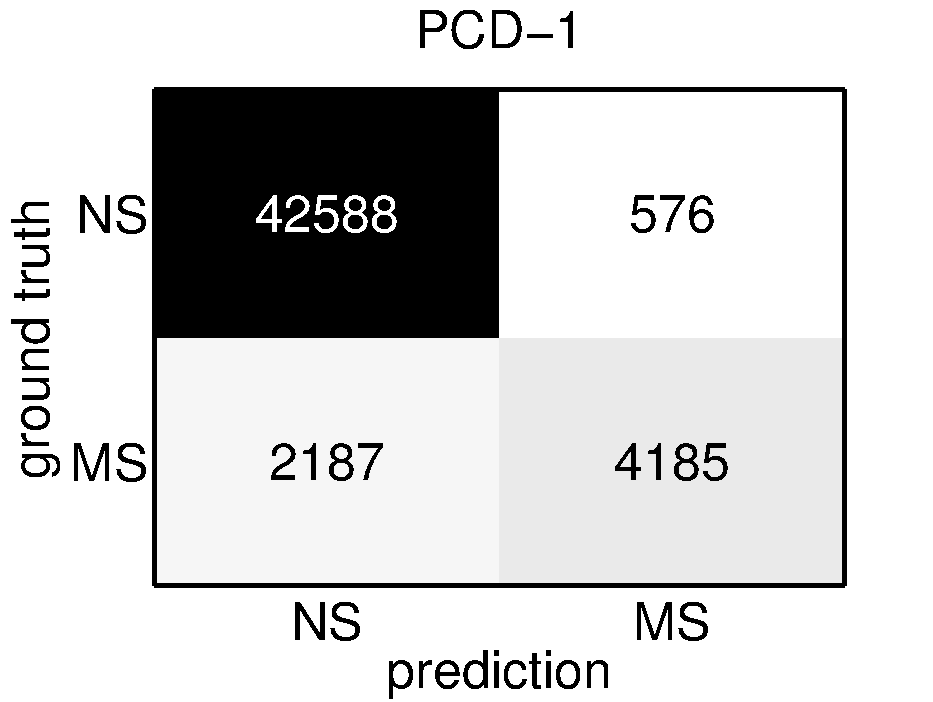
\includegraphics[width=0.48\textwidth]{./Figures/CM_PCD_1}\label{fig:CM_PCD_1}}
    \subfigure{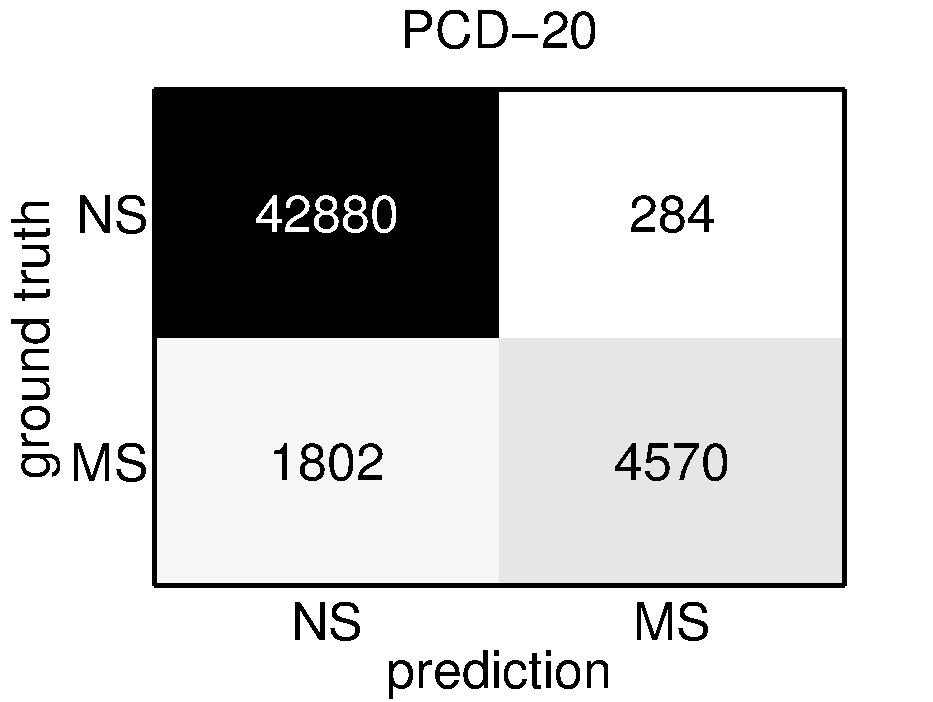
\includegraphics[width=0.48\textwidth]{./Figures/CM_PCD_20}\label{fig:CM_PCD_20}}
	\subfigure{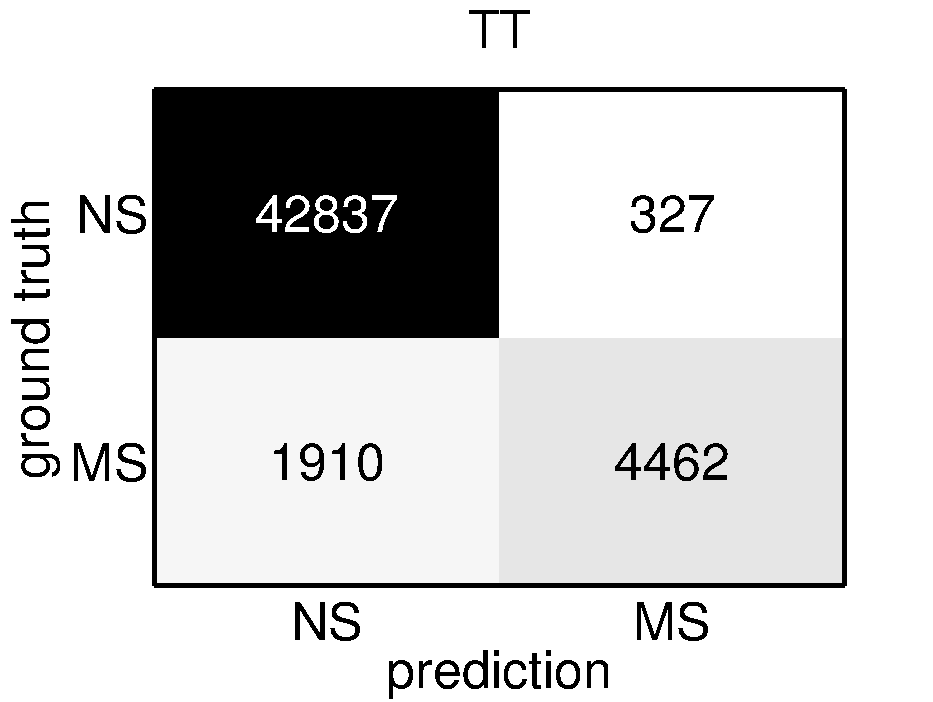
\includegraphics[width=0.48\textwidth]{./Figures/CM_TT}\label{fig:CM_TT}}
	\subfigure{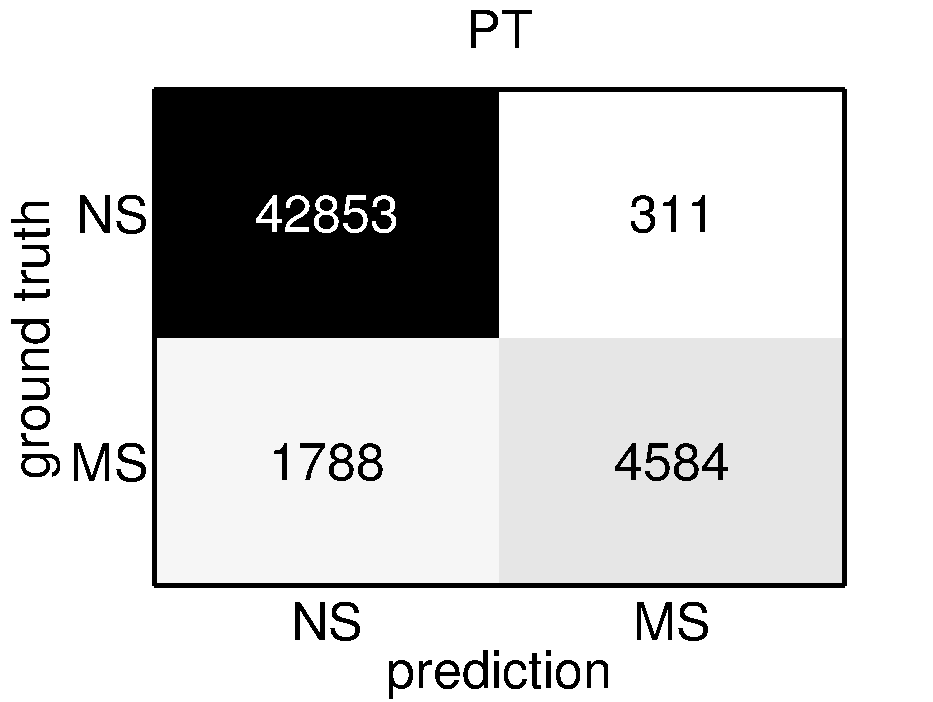
\includegraphics[width=0.48\textwidth]{./Figures/CM_PT}\label{fig:CM_PT}}
	\subfigure{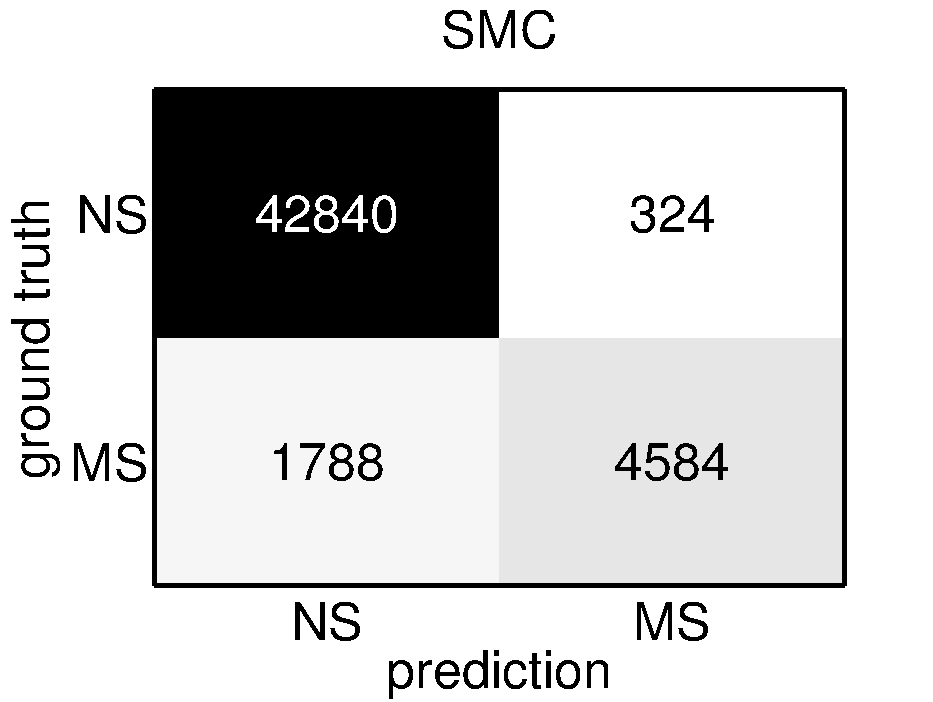
\includegraphics[width=0.48\textwidth]{./Figures/CM_SMC}\label{fig:CM_SMC}}
	\subfigure{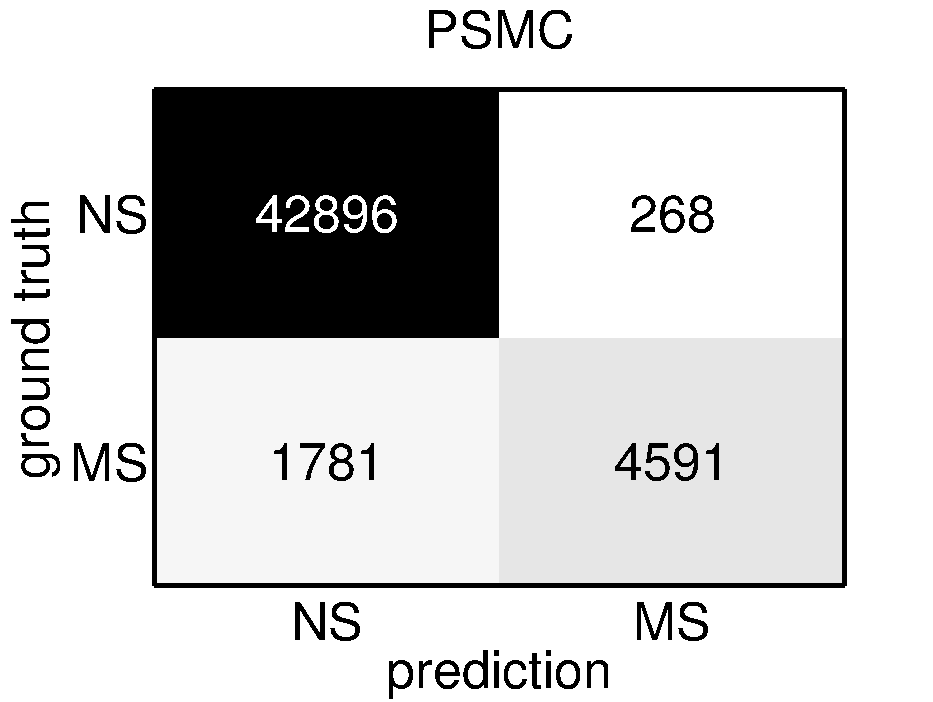
\includegraphics[width=0.48\textwidth]{./Figures/CM_PSMC}\label{fig:CM_PSCM}}
    \caption{Confusion matrices of binary segmentation by six algorithms.}   
    \label{fig:img_seg_results}
\end{figure}

\begin{figure}[t!] 
    \centering
    \subfigure[]{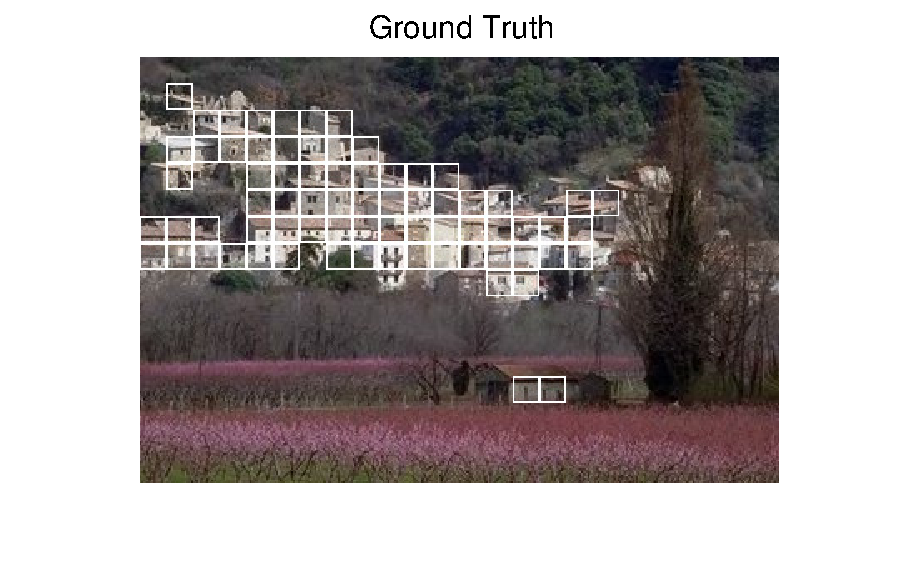
\includegraphics[width=0.7\textwidth]{./Figures/img_seg_GT}\label{fig:img_seg_GT}} \\
    \subfigure[]{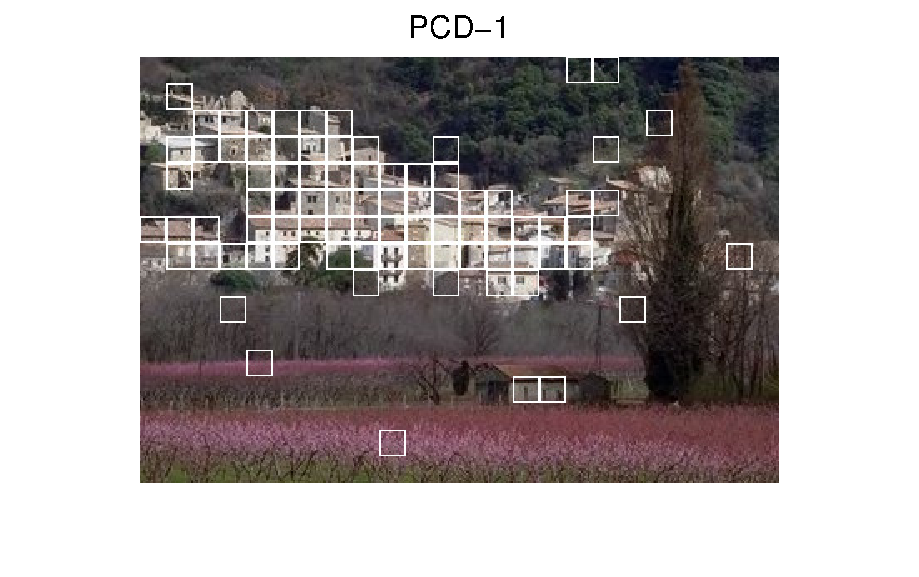
\includegraphics[width=0.49\textwidth]{./Figures/img_seg_PCD_1}\label{fig:img_seg_PCD_1}}
    \subfigure[]{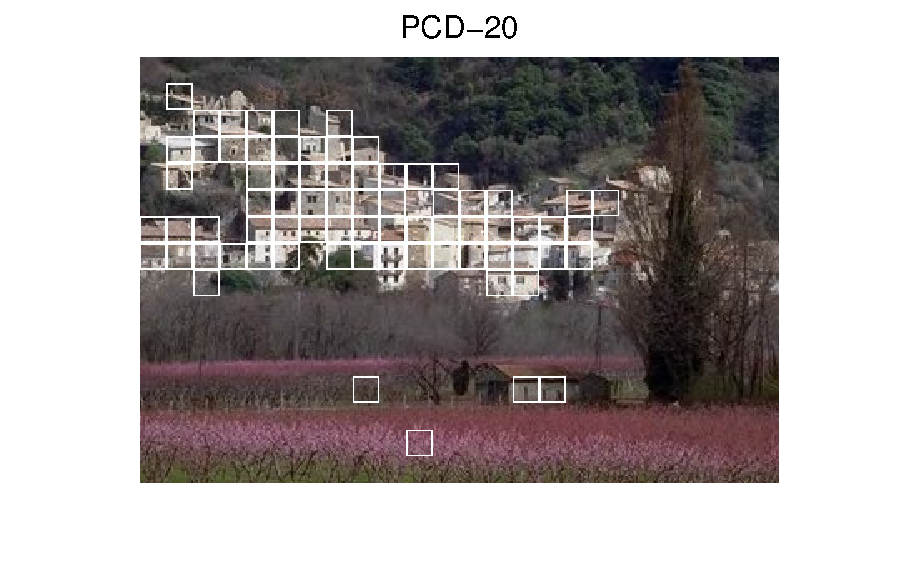
\includegraphics[width=0.49\textwidth]{./Figures/img_seg_PCD_20}\label{fig:img_seg_PCD_20}}
	\subfigure[]{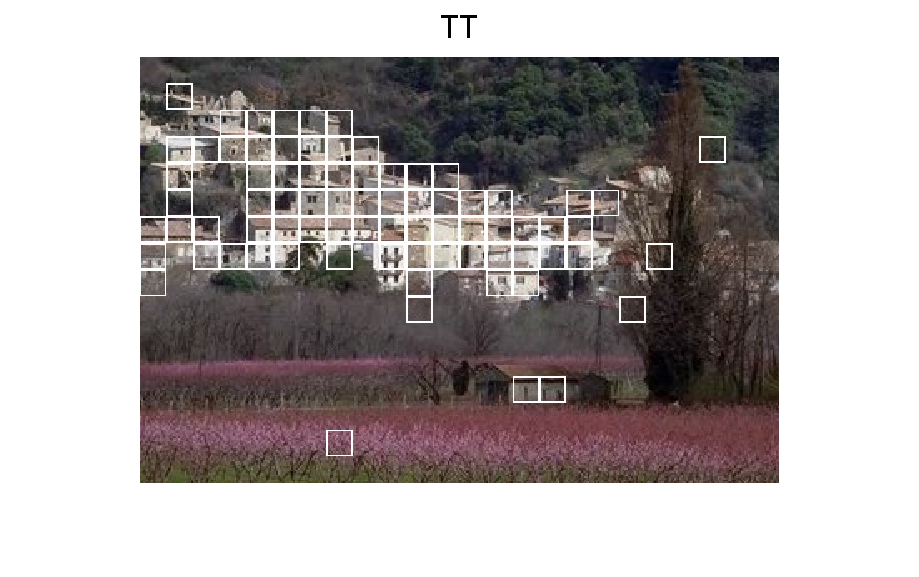
\includegraphics[width=0.49\textwidth]{./Figures/img_seg_TT}\label{fig:img_seg_TT}}
	\subfigure[]{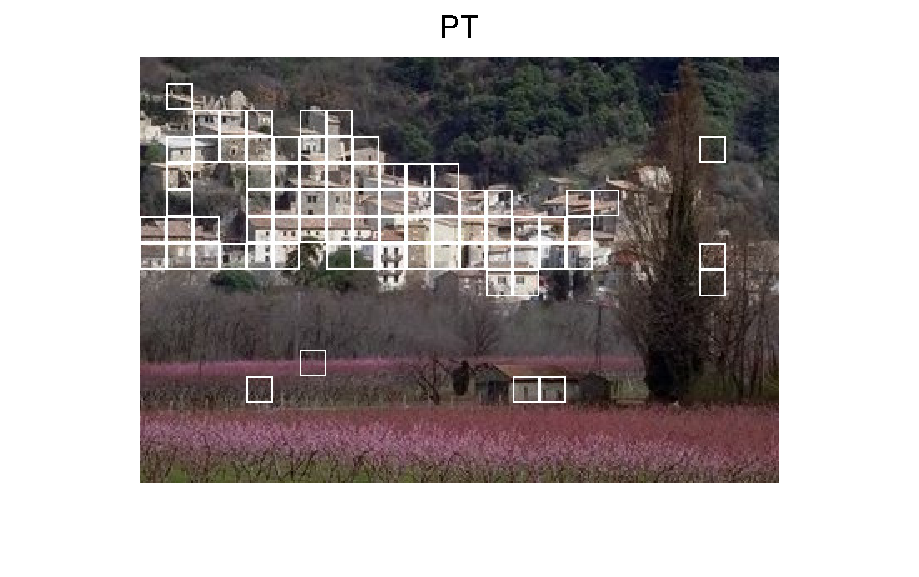
\includegraphics[width=0.49\textwidth]{./Figures/img_seg_PT}\label{fig:img_seg_PT}}
	\subfigure[]{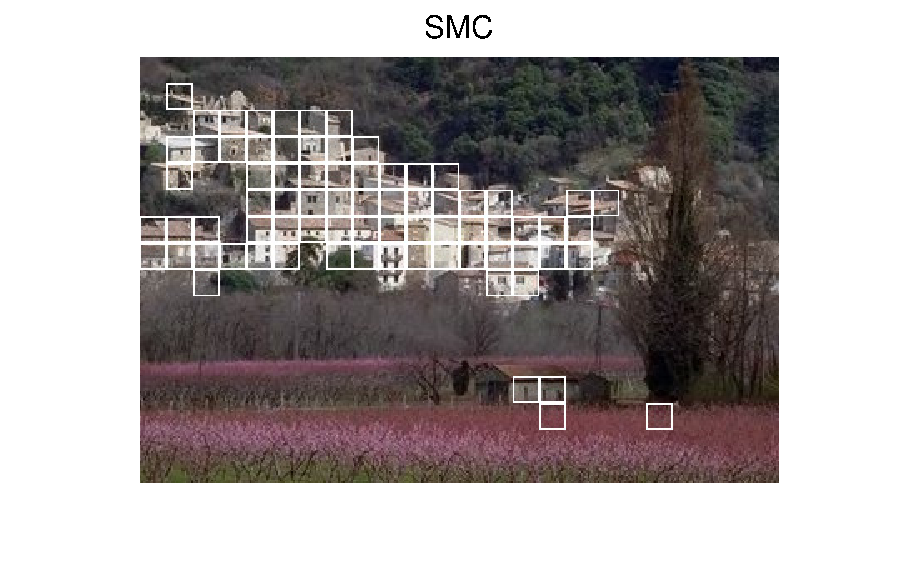
\includegraphics[width=0.49\textwidth]{./Figures/img_seg_SMC}\label{fig:img_seg_SMC}}
	\subfigure[]{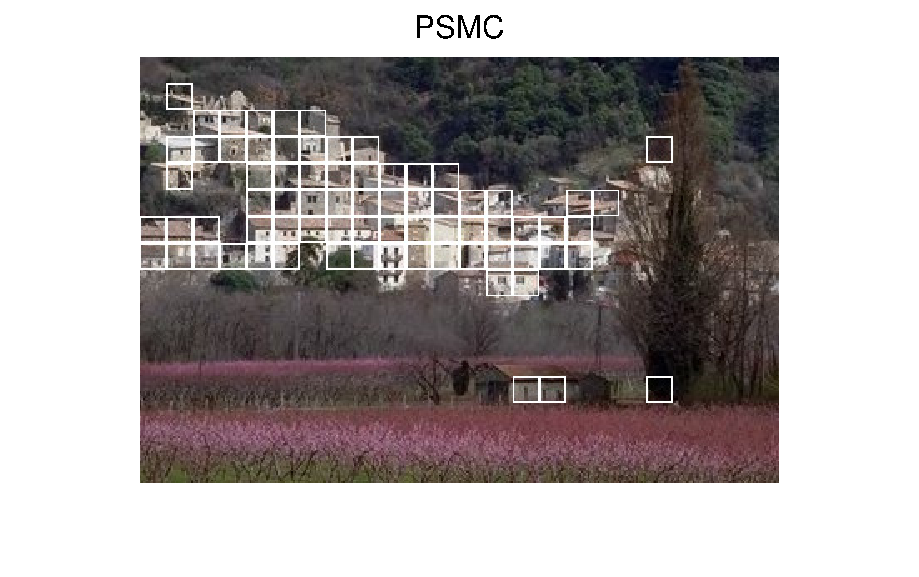
\includegraphics[width=0.49\textwidth]{./Figures/img_seg_PSMC}\label{fig:img_seg_PSCM}}
    \caption{An example image and corresponding segmentations by six algorithms.  }   
    \label{fig:img_seg_example}
\end{figure}


